%% For double-blind review submission, w/o CCS and ACM Reference (max submission space)
\documentclass[sigplan,10pt,review,anonymous]{acmart}\settopmatter{printfolios=true,printccs=false,printacmref=false}
%% For double-blind review submission, w/ CCS and ACM Reference
%\documentclass[sigplan,review,anonymous]{acmart}\settopmatter{printfolios=true}
%% For single-blind review submission, w/o CCS and ACM Reference (max submission space)
%\documentclass[sigplan,review]{acmart}\settopmatter{printfolios=true,printccs=false,printacmref=false}
%% For single-blind review submission, w/ CCS and ACM Reference
%\documentclass[sigplan,review]{acmart}\settopmatter{printfolios=true}
%% For final camera-ready submission, w/ required CCS and ACM Reference
%\documentclass[sigplan]{acmart}\settopmatter{}
\usepackage{amsmath}
\usepackage{xspace}
\usepackage{natbib}
\usepackage{csvsimple}
\usepackage{microtype}
\usepackage{tikz}
\usepackage{tikz-qtree}
\usepackage{tabularx}
\definecolor{uwpurple}{RGB}{128,0,128}
\newcommand{\jln}[1]{\textcolor{uwpurple}{\textit{[{#1} --JLN]}}}
\newcommand{\sak}[1]{\textcolor{olive}{\textit{[{#1} --SK]}}}
\usepackage{syntax}
%% Conference information
%% Supplied to authors by publisher for camera-ready submission;
%% use defaults for review submission.
\acmConference[PLDI'20]{ACM SIGPLAN Conference on Programming Language Design and Implementation}{June 2020}{London, UK}
\acmYear{2020}
\acmISBN{} % \acmISBN{978-x-xxxx-xxxx-x/YY/MM}
\acmDOI{} % \acmDOI{10.1145/nnnnnnn.nnnnnnn}
\startPage{1}

%% Macros for quantities
\newcommand{\NumApps}{{\color{red} 7}\xspace}
\newcommand{\NumRulesFixed}{{\color{red} 4}\xspace}
\newcommand{\NumPredicatesRelaxed}{{\color{red} XX}\xspace}
\newcommand{\NumOrderingProblems}{{\color{red} 46}\xspace}
\newcommand{\NumRulesSynthesized}{{\color{red} XX}\xspace}
\newcommand{\NumFailureExamples}{{\color{red} XX}\xspace}
\newcommand{\NumBugsAutomated}{{\color{red} 5}\xspace}



%% Copyright information
%% Supplied to authors (based on authors' rights management selection;
%% see authors.acm.org) by publisher for camera-ready submission;
%% use 'none' for review submission.
\setcopyright{none}
%\setcopyright{acmcopyright}
%\setcopyright{acmlicensed}
%\setcopyright{rightsretained}
%\copyrightyear{2018}           %% If different from \acmYear

%% Bibliography style
\bibliographystyle{ACM-Reference-Format}
%% Citation style
%\citestyle{acmauthoryear}  %% For author/year citations
%\citestyle{acmnumeric}     %% For numeric citations
%\setcitestyle{nosort}      %% With 'acmnumeric', to disable automatic
                            %% sorting of references within a single citation;
                            %% e.g., \cite{Smith99,Carpenter05,Baker12}
                            %% rendered as [14,5,2] rather than [2,5,14].
%\setcitesyle{nocompress}   %% With 'acmnumeric', to disable automatic
                            %% compression of sequential references within a
                            %% single citation;
                            %% e.g., \cite{Baker12,Baker14,Baker16}
                            %% rendered as [2,3,4] rather than [2-4].


%%%%%%%%%%%%%%%%%%%%%%%%%%%%%%%%%%%%%%%%%%%%%%%%%%%%%%%%%%%%%%%%%%%%%%
%% Note: Authors migrating a paper from traditional SIGPLAN
%% proceedings format to PACMPL format must update the
%% '\documentclass' and topmatter commands above; see
%% 'acmart-pacmpl-template.tex'.
%%%%%%%%%%%%%%%%%%%%%%%%%%%%%%%%%%%%%%%%%%%%%%%%%%%%%%%%%%%%%%%%%%%%%%


%% Some recommended packages.
\usepackage{booktabs}   %% For formal tables:
                        %% http://ctan.org/pkg/booktabs
\usepackage{subcaption} %% For complex figures with subfigures/subcaptions
                        %% http://ctan.org/pkg/subcaption


\begin{document}

%% Title information
\title{Verifying and Improving Halide’s Term Rewriting System with Program Synthesis}         %% [Short Title] is optional;
                                        %% when present, will be used in
                                        %% header instead of Full Title.
%\titlenote{with title note}             %% \titlenote is optional;
                                        %% can be repeated if necessary;
                                        %% contents suppressed with 'anonymous'
%\subtitle{Subtitle}                     %% \subtitle is optional
%\subtitlenote{with subtitle note}       %% \subtitlenote is optional;
                                        %% can be repeated if necessary;
                                        %% contents suppressed with 'anonymous'


%% Author information
%% Contents and number of authors suppressed with 'anonymous'.
%% Each author should be introduced by \author, followed by
%% \authornote (optional), \orcid (optional), \affiliation, and
%% \email.
%% An author may have multiple affiliations and/or emails; repeat the
%% appropriate command.
%% Many elements are not rendered, but should be provided for metadata
%% extraction tools.

%% Author with single affiliation.
\author{First1 Last1}
\authornote{with author1 note}          %% \authornote is optional;
                                        %% can be repeated if necessary
\orcid{nnnn-nnnn-nnnn-nnnn}             %% \orcid is optional
\affiliation{
  \position{Position1}
  \department{Department1}              %% \department is recommended
  \institution{Institution1}            %% \institution is required
  \streetaddress{Street1 Address1}
  \city{City1}
  \state{State1}
  \postcode{Post-Code1}
  \country{Country1}                    %% \country is recommended
}
\email{first1.last1@inst1.edu}          %% \email is recommended

%% Author with two affiliations and emails.
\author{First2 Last2}
\authornote{with author2 note}          %% \authornote is optional;
                                        %% can be repeated if necessary
\orcid{nnnn-nnnn-nnnn-nnnn}             %% \orcid is optional
\affiliation{
  \position{Position2a}
  \department{Department2a}             %% \department is recommended
  \institution{Institution2a}           %% \institution is required
  \streetaddress{Street2a Address2a}
  \city{City2a}
  \state{State2a}
  \postcode{Post-Code2a}
  \country{Country2a}                   %% \country is recommended
}
\email{first2.last2@inst2a.com}         %% \email is recommended
\affiliation{
  \position{Position2b}
  \department{Department2b}             %% \department is recommended
  \institution{Institution2b}           %% \institution is required
  \streetaddress{Street3b Address2b}
  \city{City2b}
  \state{State2b}
  \postcode{Post-Code2b}
  \country{Country2b}                   %% \country is recommended
}
\email{first2.last2@inst2b.org}         %% \email is recommended


%% Abstract
%% Note: \begin{abstract}...\end{abstract} environment must come
%% before \maketitle command
\begin{abstract}
  The wide adoption of Halide as an efficient domain-specific language
  for image processing and tensor computations shows the language is
  useful and effective for compiling high performance code across platforms.
  In Halide, reasoning about the code relies on a term rewriting system to
  prove properties required for efficient and correct compilation.  This rewrite
  system is written as a collection of handwritten transformation rules 
  that incrementally rewrite expressions into simpler forms and requires high performance 
  in both time and memory usage to keep compile times low.
  In this work, we apply formal techniques to prove the correctness of existing
  rewrite rules and provide a guarantee of termination. Then,
  we build an automatic program synthesis system that learns new, provably
  correct rules from failure cases where the compiler was unable to prove properties. We
  identify and fix \NumRulesFixed incorrect rules as well as \NumOrderingProblems rules
  which could give rise to infinite rewriting loops. We run our synthesis process against 
  a large suite of failed proofs from realistic applications, discovering \NumRulesSynthesized new rules. 
  The automated system can replace tedious human effort required to craft new rules
  in response to user-reported bugs.  We demonstrate that the new
  term rewriting system is more correct, more robust, and more general, without
  making compilation time slower.
\end{abstract}


%% 2012 ACM Computing Classification System (CSS) concepts
%% Generate at 'http://dl.acm.org/ccs/ccs.cfm'.
\begin{CCSXML}
<ccs2012>
<concept>
<concept_id>10011007.10011006.10011008</concept_id>
<concept_desc>Software and its engineering~General programming languages</concept_desc>
<concept_significance>500</concept_significance>
</concept>
<concept>
<concept_id>10003456.10003457.10003521.10003525</concept_id>
<concept_desc>Social and professional topics~History of programming languages</concept_desc>
<concept_significance>300</concept_significance>
</concept>
</ccs2012>
\end{CCSXML}

\ccsdesc[500]{Software and its engineering~General programming languages}
\ccsdesc[300]{Social and professional topics~History of programming languages}
%% End of generated code


%% Keywords
%% comma separated list
\keywords{keyword1, keyword2, keyword3}  %% \keywords are mandatory in final camera-ready submission


%% \maketitle
%% Note: \maketitle command must come after title commands, author
%% commands, abstract environment, Computing Classification System
%% environment and commands, and keywords command.
\maketitle


\section{Introduction}
Tensor and image processing pipelines power a large number of applications,
including computational photography, medical imaging, machine learning,
and computer vision, which run on a large variety of platforms, from
mobile phones to large-scale servers in the cloud.  For many of these
applications, high performance is an essential requirement due to real-time
requirements, compute cost, and battery life.

Halide~\cite{ragankelley2012halide, ragankelley2013halide} has proven to be an effective
domain-specific language for writing such code and obtaining cross-platform
high performance, with multiple industrial vendors relying on Halide to power
applications used by millions of users on mobile phones, tablets, desktops, and
servers.  Halide separates what is computed (the \textit{algorithm}) from how
the computation executes (the \textit{schedule}); the compiler ensures that
different schedules for different platforms correctly compute the algorithm.
Schedules often require the compiler to prove specific properties in order
to guarantee correctness or to ensure the resulting code performs as well
as possible.  For example, to fully unroll a loop, the compiler must prove
the loop has a constant extent.

Many of these properties relate regions of computation with one another,
which, within Halide, are represented as intervals over the integers.
Reasoning about these regions uses a \textit{term rewriting system}
(TRS) on integers: the compiler applies simplification rules to an expression relating
the regions until no more rewrites apply.  The final expression can be
true, false, or some more complex expression. If an expression is semantically equivalent to true,
but the simplifier cannot rewrite it to that form, it may be unable to apply a valid optimization,
resulting in suboptimal code output and possibly errors during compilation.

In this work, we improve the Halide term rewriting system by formally checking the existing
set of rules to ensure correctness, and then constructing a rule ordering that 
ensures termination.  We then automate the task of writing new rules by building a program
synthesis system that automatically checks compilation failures for expressions that are
correct but not provable, and produces new rules with predicates to guard their application.
These new rules will preserve correctness and termination properties by construction.

An ideal TRS for our purpose would fully express the semantics of the Halide expression language and be \emph{convergent}, meaning that if two expressions are equivalent,
the TRS will return the same canonical form for both of them. If so, the simplifier could take any two expressions and determine if they were equivalent by rewriting them and checking to see if they have the same form. However, constructing such a TRS is impossible. Suppose we had a finite set of equational identities $E$ that fully express all the properties of the Halide expression language. A convergent TRS equivalent to $E$ would need to be \emph{convergent}, meaning that if an expression can be rewritten in multiple ways, it will ultimately arrive at the same form, and \emph{terminating}. However, we know $E$ must contain identities that are fundamentally non-terminating, such as commutative properties like $x * y \equiv y * x$. Furthermore, since the Halide expression language contains nonlinear integer arithmetic, the problem of constructing $E$ itself is undecidable. Thus, the challenge for the Halide TRS is to be able to reason about as much of the Halide expression space as it can, while remaining deterministic and performant.

In Halide's compiler, the TRS consists of a series of
handwritten rules and efficient matchers to match rules bottom-up.  These rules were constructed
by developers based on observed compilation failures over many years, and ordered in ad-hoc ways
to avoid non-termination.  Extensive fuzz-testing has been able to find bugs in rewrite rules,
but fuzz-testing cannot provide formal guarantees (and in fact we were able to find bugs in the current version of the simplifer; see~\ref{sec:eval-correctness}). Furthermore, adding additional
rules requires expert programmers to meticulously analyze compilation failures and hand-craft
rules that mitigate the problems without causing new errors.

The verification and synthesis
of these rules poses significant challenges: the underlying theory of non-linear integer arithmetic (NLIA)
is known to be undecidable~\cite{matiyasevich1993hilberts10th}. We verify
existing rules using a combination of the Z3~\cite{de2008z3} satisfiability
modulo theory (SMT) solver and the Coq~\cite{coq19} interactive theorem prover. 
New rules are constructed by combining Z3 and a hand-written solver that uses beam
search with a learned cost model. To search for cases where the Halide compiler
fails to prove properties, we run \NumApps existing Halide pipelines with
randomized schedules, and augment this set with a random pipeline generator
designed to produce plausible image processing and machine learning pipelines.
\sak{Revise previous sentence if we can gety by with just random pipelines}

We make three main contributions:
\begin{itemize}
  \item We guarantee soundness by verifying the existing Halide TRS.
  \item We guarantee termination by fixing a reduction order.
  \item We strengthen the simplifier by developing a synthesis algorithm to learn new rewrite rules from expressions the current simplifier cannot make progress on.
\end{itemize}

Overall, we discover \NumRulesFixed bugs in hand-written Halide simplifier rules, and discover \NumOrderingProblems
potential issues in rule ordering.  We then synthesize \NumRulesSynthesized new rules from \NumFailureExamples
failure examples and further demonstrate the utility of our synthesizer by attempting to
automatically produce the \NumBugsAutomated latest code changes that add new
rules based on compiler misbehavior. We additionally craft a strategy for grouping
new rules that prevents compile times from increasing linearly with the number
of rules.  Overall, we demonstrate that our approach
reduces compilation failures, does not slow down the compiler, and replaces the
tedious human effort required to craft bug fixes due to missing rules in the
term rewriting system.

\section{Overview}
\subsection{Term Rewriting Systems}
Term rewriting systems~\cite{gorn1967} successively apply \textit{rewrite rules} to transform a given
expression into a simpler form, until no further simplifications are possible.  Such systems are widely
used in theorem proving~\cite{} and abstract interpretation~\cite{}.

Terms are defined inductively over a set of variables $V$ and a set of function symbols $\Sigma$. Every variable $v \in V$ is a term, and for any function symbol $f \in \Sigma$ with arity $n$ and any terms $t_1, ..., t_n$, the application of the symbol to the terms $f(t_1, ..., t_n)$ is also a term. We refer to the set of terms constructed from the variables $V$ and the function symbols $\Sigma$ as $T(\Sigma, V)$.

A \emph{rewrite rule} is a directed binary relation $l \rightarrow r$ such that $l$ is not a variable, and all variables present in $r$ are also present in $l$ (i.e., $\mathcal{V}ar(l) \supseteq \mathcal{V}ar(r)$). A set of rewrite rules is a \emph{term rewriting system}.

Consider a set of terms $T(\Sigma, V)$ such that $\Sigma = \{\clubsuit, \diamondsuit\}$ and $V$ is an infinite set of variables. Let the term rewriting system $R$ consist of a single rule:

\[ R = \{ x_1 \clubsuit x_2 \rightarrow_R x_1 \diamondsuit x_2 \} \]

We use $R$ to rewrite the term

\[ 
(y_1 \diamondsuit y_1) \clubsuit (y_2 \clubsuit y_3)
\]

The first step is matching; we find a substitution that will unify the lefthand side (LHS) of the rule with the term we are rewriting. Here, the substitution is:

\[
\{ x_1 \mapsto (y_1 \diamondsuit y_1), x_2 \mapsto (y_2 \clubsuit y_3) \}
\]

We then apply this substitution to the righthand side (RHS) of the rule to obtain the rewritten version of the original term.

\[ 
(y_1 \diamondsuit y_1) \diamondsuit (y_2 \clubsuit y_3)
\]

\begin{figure*}
\begin{tabularx}{\textwidth}{XXXX}
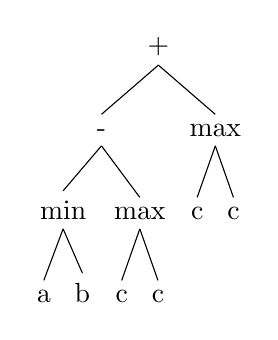
\begin{tikzpicture}
\Tree [.+ [.- [.min a b ] [.max c c ] ] [.max c c ]]
\end{tikzpicture}
&
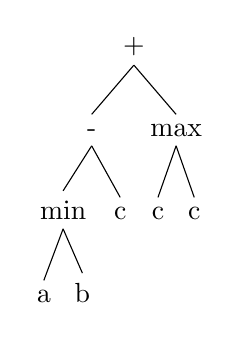
\begin{tikzpicture}
\Tree [.+ [.- [.min a b ] c ] [.max c c ]]
\end{tikzpicture}
&
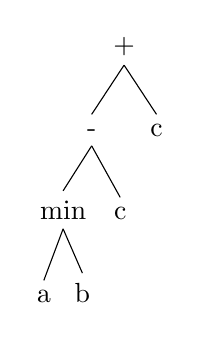
\begin{tikzpicture}
\Tree [.+ [.- [.min a b ] c ] c ]
\end{tikzpicture}
&
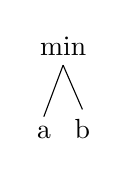
\begin{tikzpicture}
\Tree [.min a b ]
\end{tikzpicture}
\end{tabularx}
\caption{We demonstrate the Halide simplifier algorithm using a TRS $R = \{max(x,x) \rightarrow_R x, (x - y) + y \rightarrow_R x\}$ and an expression $min(a,b) - max(c,c) + max(c,c))$. The algorithm attempts to simplify all subtrees bottom up; here, no rule applies to $min(a,b)$ so it is not changed. Next, rule 1 rewrites $max(c,c)$ to $c$. No rule applies to $min(a,b) - c$, so we move to the rightmost subtree and rewrite again to obtain $c$ from $max(c,c)$. Finally, we consider the entire tree $(min(a,b) - c) + c$ and apply rule 2 to produce $min(a,b)$. No rules match this expression, so we are done. \jln{nicer formatting TK}}
\label{fig:algoexample}
\end{figure*}

\subsection{Term Rewriting in Halide}

The Halide compiler contains a term rewriting system, currently composed of
several hundred rules, that operates over the space of Halide
expressions\footnote{See Appendix ~\ref{ss:appendixA} for the full Halide
  expression grammar}. While the term rewriting system is used for multiple
purposes within the compiler, the two most important
uses are when the TRS serves proof engine to determine if
some equality or inequality holds, or when the rewriter attempts to find tight
bounds on regions. For example, in order to parallelize a
reduction variable, the compiler must prove that there are no hazards, which is
done using the TRS as proof engine.  Another example is that Halide uses
the TRS to decide how much memory to allocate for intermediates; tighter, more
simplified bounds result in more efficient execution since they eliminate over-allocation.
More generally, proof engine failures can lead to:
\begin{itemize}
\item Insufficiently tight bounds on loops and allocations, which may result in
  runtime failures (e.g. due to memory overallocation) or performance issues;

\item Failure of the compiler to apply optimizations, also resulting in slow performance;

\item Dynamic checks in the generated code, for properties that could have been proven
  at compile time, leading to slower code;

\item Compilation failures, when the compiler is unable to correctly produce code
  even though the properties required hold, or when the proof engine itself crashes
  or loops infinitely.
\end{itemize}
Thus, correctness and generality are essential to make the compiler robust and
able to generate fast code.

The design of the term rewriting algorithm has two additional important
requirements. The first is performance: although the TRS is called at
compile time, it may be invoked over a hundred thousand times in compiling a single pipeline
Thus, unlike many term rewriting algorithms, the Halide TRS
never backtracks and must be careful about memory usage. The second requirement is determinisim: the compiler must
always return the same schedule every time it encounters a particular pipeline.
This precludes any non-deterministic search strategy for the best sequence of
rules to apply, or directly invoking a solver such as Z3, since even with a
fixed random seed, machines with different computational power may return
different results within a given timeout.

The Halide term rewriting algorithm simplifies an input expression in a
depth-first, bottom-up traversal of the expression DAG. At each node, it looks
up the list of rewrite rules that correspond to the node's function symbol, then
attempts to match the subtree expression with the rule LHSs in order. When a
match is found, it rewrites the subtree expression using the RHS of that rule,
and then attempts to simplify the subtree expression again. If no rule matches
the subtree, the traversal continues; when the entire expression cannot be
simplified further, the rewritten expression is returned. See figure~\ref{fig:algoexample} for a worked example. 
In the worst case, the performance of this algorithm is exponential since it attempts to match rewrite rules for every subtree of the expression AST. However, the fact that the algorithm never backtracks gives important performance advantages (see below).

Halide rewrite rules optionally contain a compile-time predicate that must hold for a rule to
be applied. Halide expressions may contain constants whose values are known at
compile time. Predicate expressions contain only such constants; when the
LHS of a rule matches an expression, its predicate is evaluated and only if it
is true will the rewrite be applied.

We limit ourselves to expressions over the set of infinite precision integers in
this work, although Halide expressions can contain floats and fixed-width
integers. However, the uses of the TRS we consider in this work all operate
on infinite integers.

\subsection{Why a custom algorithm?}

Given that we make use of the Z3 solver as an oracle for both verification and synthesis, it is natural to ask why Halide could not simply call Z3 for simplification. Z3 is the product of extensive development and is a very powerful, general-purpose solver. However, the Halide simplifier has a few key properties that Z3 does not: deterministic output, low memory and compute requirements, and domain-specific optimizations.

The Halide compiler must return the same schedule every time the same pipeline is run. Z3 can fix a random seed, but long-running queries may be able to complete on a more powerful server when it might time out on another.

A more usual term rewriting algorithm would use backtracking search; at any given step in the rewriting process, multiple rules may match a given expression, and the algorithm must pick one to explore. If that choice was not fruitful, the algorithm will backtrack and choose another path. The Halide simplifier algorithm never backtracks; rules are assigned a fixed priority, and the algorithm applies the first rule that matches in that priority order. This makes the simplifier memory efficient, since it only persists the single expression it is in the process of rewriting, without the checkpoints or equivalence classes that would be necessary for a backtracking search. The tradeoff is that the Halide algorithm may pick the ``wrong'' rule and have no way of undoing that decision. Since the simplifier is invoked many thousands of times with each call of the compiler, it chooses to sacrifice some solving power in exchange for performance. This choice gives the Halide algorithm a very smooth performance curve, whether it succeeds or fails in simplifying an input expression, while a solver like Z3 tends to give very good performance in the majority of cases but get bogged down in difficult cases, requiring the use of timeouts. \jln{should be able to add a graph showing z3 vs simplifier performance on expression suite demonstrating this}

This also means that the Halide algorithm scales very well in terms of the number of rules in the TRS, whereas adding rules to a more usual backtracking search algorithm causes its search space to grow exponentially. See section~\ref{ssec:compilationspeed} for an evaluation of the effects of adding newly synthesized rules on the performance of the compiler. 

Finally, although Z3 can be used to simplify expressions, its cost metric is to simply reduce the size of expressions. Gathering like terms in some cases can actually prevent Halide or LLVM optimizations from applying. The Halide simplifier guides expressions into more optimizable forms and can be changed or tuned as needed if further optimizations are discovered. \jln{should also mention here that Halide simplifier can solve some expressions that z3 cannot, as shown by the fact that z3 could not verify around 100 of the rewrite rules}

%Z3 is general-purpose, but we need not be. The handwritten simplifier ruleset was written to address expressions that are generated by the Halide compiler. Since we are driven by a subset of all Halide expressions and not arbitrary expressions in the Halide expression language, we can specialize and in some cases solve expressions that Z3 cannot. 


%Egraphs grow their equivalence classes with each invocation of their rulesets until they converge or until their graph grows so large that progress is no longer possible. Since we can't guarantee that our rules converge, the problem is reaching the goal state before the growth of the graph reaches that infeasible inflection point.

%Egraph handling of predicates is also more computationally expensive than the Halide TRS; Halide evaluates constants at compile time to see if a predicate obtains on a particular expression. Since egraphs have no knowledge of semantics, the machinary for handling predicates is much more involved.

%If bounded, egraphs are also deterministic, so that's not a problem.

%I know that dumping the Halide ruleset into an egraph is completely unworkable, since I tried it -- not a fair comparsion since you would tune an egraph's ruleset differently.

%The Halide TRS gives a nice starting point for synthesis because a failed call to the simplifier yields an expression the simplifier can make no progress on. A failed egraph call gives an equivalence class that should include the goal state but doesn't, so it's not as clear how to debug that.

\subsection{Program Synthesis}
Syntax-guided synthesis (SyGuS)~\cite{sygus} has been used
to search over a space of possible programs in order to find one that meets
a semantic specification.  One of the most popular techniques is counterexample-guided
inductive synthesis (CEGIS), which leverages the power of satisfiability modulo theories
(SMT) and SAT solvers to make search over a large space of programs more intelligent.
In CEGIS, the task is to find some program in the search space such that for all possible
inputs, the found program fulfills some semantic criteria, usually equivalence with
a specification.

The CEGIS process proceeds in a loop. Given a specification $S$ and arbitrary
settings for $C = {c_0,..c_i}$, constructing a query to the SMT engine that searches for
a counterexample to equivalence:
$$\forall B, \neg (f(C, B) = S(B))$$
The solver either returns unsatisfiable, meaning the the choices encoded in $C$
indeed result in a program equivalent to $S$, or returns a counterexample input $e_0$
for which the two programs give different results.  Then, the CEGIS system constructs a new query,
asking the SMT solver for choices $C'$ such that the two programs are equivalent for just the
counterexample input.
Given the $C'$ returned by the solver, CEGIS then attempts the original query once again, to
determine whether the returned program generalizes to all inputs.
If another counterexample $e_1$ is found, another iteration of the CEGIS loop begins, this time querying
the solver for $C'$ that results in equivalent behavior to $S$ for both counterexample inputs.
In this manner, the CEGIS loop iterates between querying the solver for new $C'$ valid
for all found counterexamples so far, then queries the SMT solver to prove the new $C'$ is
correct for all inputs.  The loop terminates when the final $C'$ is proven correct for
possible inputs or if no setting of $C$ can make the programs equivalent.

\section{Soundness}
\label{sec:soundness}

We improve the Halide term rewriting system by ensuring its soundness in
two ways: first, we verify that each individual rule is correct, meaning the
rewrite preserves semantics. Then we verify that the term rewriting system is
guaranteed to terminate on all inputs by ensuring that there is no sequence of
applications of rules, on any input expression, that can form a cycle.

\subsection{Rule verification}

We verify each individual rule is correct by modeling Halide expressions in SMT2
and using the SMT solver Z3~\cite{de2008z3} to prove that the rule equivalences must hold.
Most Halide expression semantics map cleanly
to SMT2 formulas. The functions \texttt{max} and \texttt{min} are defined in
the usual way, and \texttt{select} in Halide is equivalent to the SMT2 operator
\texttt{ite}. Division and modulo are given the Euclidean definitions in both
Halide and SMT2~\cite{boute1992euclidean}. If a variable appears in the LHS of a rule as a divisor in a
division or modulo operation, it is assumed to be non-zero. %The Halide
%expressions do not have a true boolean type (true and false are represented by
%unsigned integers of 1 bitwidth), so expressions must be typed as either
%\texttt{Int} or \texttt{Bool} when translated into SMT2. The Halide expression
Halide contains two vector-only operators, \texttt{broadcast} and \texttt{ramp}; all
other integer operators can be coerced to vector operators. 
\texttt{broadcast} projects some value $x$ to a vector of length $l$; because of
the type coercion, we can simply represent \texttt{broadcast(x)} as the variable
\texttt{x} in SMT2. \texttt{ramp} creates a vector of length $l$
whose initial entry has the value $x$ and all subsequent entries increase with
stride $s$. In SMT2, we represent this term as the symbolic expression $x + l *
s$, where $l$ must be zero or positive.

Given this modeling, for each rule, we assert any assumptions are true, then
ask Z3 to search for a variable assignment such that the LHS and RHS are not
equivalent.  If Z3 indicates no such assignment exists, the LHS must be equivalent to
the RHS and the rule must be correct. We implemented a SMT2 printer for the
Halide rewrite rules that constructs a verification problem for each rule
suitable for passing to Z3 or other SMT system.  Rule verification using Z3 is fully automated
and can be run for the current set of rewrite rules via script.

However, nonlinear integer arithmetic is undecidable, and for 123
rules, Z3 either timed out or returned unknown. Nearly all of these rules used
either division or modulo. We used the proof assistant Coq to manually prove or
disprove the correctness of these remaining rules. \jln{about 20 left to go} We
were also able to relax the predicates of \jln{TK} rules; for example, in some cases a rule
with a predicate requiring some constant to be positive would be equally valid
if the constant was non-zero.

We further want to guarantee that, given an input expression with well-defined
behavior, the term rewriting system will never rewrite it into an expression that has
undefined behavior. For example, if an input expression never divides by zero, then the
TRS output must never divide by zero. We check this by
verifying that all terms used as divisors or moduluses in the RHS of a
rewrite rule also appear as a divisor in the rule's LHS. Note that all divisor
terms on the LHS side are not required to appear in the RHS; if a divisor is
factored out, then it is possible that the input expression would have caused a
divide-by-zero fault but the simplified expression will not. \jln{talk about
  overflow here}

Overall results of verifying rule correctness are described in Section~\ref{sec:eval-correctness}.

\subsection{Termination}

Term rewriting systems are not guaranteed to terminate. Consider a term
rewriting system containing only one rule: $x + y \rightarrow y + x$. The term
$3 + 5$ matches the LHS of the rule and is rewritten to $5 + 3$, which can again
be matched to the rule and rewritten to $3 + 5$, and so on. To guarantee
termination regardless of the rule application algorithm, every application of
a rule needs to strictly (monotonically) decrease in some measure. In other
words, we need $s \rightarrow_R t$, $s > t$ for some strict order $>$. However, since
the set of terms is infinite, we cannot check that $s > t$ for all pairs of
terms $s, t$. Instead, we show that for every rule $l \rightarrow_R r$ in our
term rewriting system, $l > r$. This will suffice if $>$ is a \emph{reduction
  order}. We take the definition of a reduction order and the next two theorems from Baader and Nipkow~\cite{baader1999term}

\begin{theorem}\label{theorem:terminates}
A term rewriting system $R$ terminates iff there exists a reduction order $>$ that satisfies $l > r$ for all $l \rightarrow_R r \in R$.
\end{theorem}

A reduction order is defined as follows.

\begin{definition}
A strict order on terms $T(\Sigma, V)$ is a reduction order iff it is: 
\begin{enumerate}
    \item well-founded, meaning that every non-empty set has a least element with regard to the order,
    \item compatible with $\Sigma$-operations: for all $s_1, s_2 \in T(\Sigma,V)$, all $n \geq 0$, and all $f \in \Sigma^{(n)}$, $s_1 > s_2$ implies
    \[ f(t_1,...t_{i-1},s_1,t_{i+1},...,t_n) > f(t_1,...t_{i-1},s_2,t_{i+1},...,t_n)
    \]
    for all $i, 1 \leq i \leq n$ and all $t_1,...t_{i-1},t_{i+1},...,t_n \in T(\Sigma,V)$.
    \item closed under substitution: for all $s_1, s_2 \in T(\Sigma,V)$ and all substitutions $\sigma \in \mathcal{S}ub(T(\Sigma,V))$, $s_1 > s_2$ implies $\sigma(s_1) > \sigma(s_2)$.
\end{enumerate}
\end{definition}

We provide a guarantee that the Halide TRS will always terminate by fixing a
reduction order over the existing ruleset. To choose our reduction order, we
need to consider the two purposes of the Halide TRS. When using the TRS
as a prover, to determine if two expressions are equivalent, we want
the output expressions to be as close to some normal form as possible, but it
doesn't particularly matter what that form is. When we use the Halide TRS
to reduce the size of an expression, however, the form of the output expression
can have strong performance implications.
Simplifying an expression in a way that
improves performance could mean cancelling correlated subexpressions, using
fewer expensive operations such as vector operations, or clustering constants
that can pre-computed into a single constant.

Consider the space of all possible Halide expressions, in which our starting
expression is a point. If all rewrite rules obey a reduction order, applying any
rewrite rule will move the expression through the expression space monotonically
in some direction, preventing cycles and ensuring termination. Our reduction
order guides the rewritten expression to some desirable part of the
expression space, but defining that desirable space is quite complex. In order
to do this, we make use of the following fact~\cite{baader1999term}:

\begin{theorem}
The lexicographic product of two terminating relations is again terminating.
\end{theorem}

Our reduction order is thus a composition of several reduction orders, each of
which moves the expression in some desirable direction. Let $>_a$ and $>_b$ be
two reduction orders; the lexicographic product of those orders $>_{a \times b}$
is:

\[
s >_{a \times b} t \iff s >_a t \vee (s \geq_a t \wedge s >_b t)
\] 

In other words, given an order $>_{a \times b}$, our rewrite system is allowed
to move the expression monotonically in the direction of $>_a$, and
monotonically in the direction of $>_b$ only as long as the $>_a$ order is not
violated.

Our component reduction orders have three main types: orders over variable
occurrence counts, orders over operation occurrence counts, and recursive
multiset path orders. We sketch the proof that the orders have the required
properties for reduction orders in the remainder of this section; a full
definition of the reduction order is given in Appendix ~\ref{a:reductionorder}.

First, orders over variable or operation occurrence counts are well-founded 
because they are defined using a measure function that maps terms to the natural
numbers. Let the function $|s|_x$ represent the number of occurrences of the
variable $x$ in the term $s$. Similarly, let $|s|_f$ represent the number of
occurrences of some symbol $f \in \Sigma$ in the term $s$. Thus, we can define a reduction order such that for every variable present in some term $s$, that variable occurs strictly more times in $s$ then in term $t$.

\begin{equation*}
s >_{var} t \iff \forall x \in V, |s|_x > |t|_x
\end{equation*}

The order is compatible with $\Sigma$-operations, as is any order based on the number of occurrences of variables or operations. For terms $s$ and $t$, let $s' = f(u_1,...u_{i-1},s,u_{i+1},...,u_n)$ and $t' = f(u_1,...u_{i-1},t,u_{i+1},...,u_n)$. Then, 

\begin{gather*}
|s'|_x = \sum_{u_j}^{0<j<=(i-1)} |u_j|_x + |s|_x + \sum_{u_j}^{(i+1)<j \leq n} |u_j|_x \\
|t'|_x = \sum_{u_j}^{0<j<=(i-1)} |u_j|_x + |t|_x + \sum_{u_j}^{(i+1)<j \leq n} |u_j|_x
\end{gather*}

As the summations are the same for $|s'|_x$ and $|t'|_x$, it must be true that if $|s|_x > |t|_x$, then $|s'|_x > |t'|_x$.

The order is also closed under substitution; for any variable substitution
$v \mapsto u$, the number of occurrences of any variable $x$ will be increased
by some $n = |u|_x$ for every occurrence of $v$ in $s$. Since we know $v$ occurs
fewer times in $t$ than $s$, the relation must hold.

We use similar orders defined using the number of occurrences of function symbols in terms. As an example consider an order $>_{\texttt{\%}}$ which states that $s >_{\texttt{\%}} t$ if $s$ contains strictly more modulo operations than $t$. This order is compatible with $\Sigma$-operations by the same argument as above. We need to add one more condition to make sure this order is closed under substitution:

\begin{equation*}
s >_{\texttt{\%}} t \iff |s|_{\texttt{\%}} > |t|_{\texttt{\%}} \wedge \forall x \in V, |s|_x \geq |t|_x
\end{equation*}

If $t$ contains more occurrences of some variable $v$ than $s$, some substitution $v \mapsto u$ such that $|u|_{\texttt{\%}} > 0$ would increase the size of $|\sigma(t)|_{\texttt{\%}}$ more than it would the size of $|\sigma(s)|_{\texttt{\%}}$. By fixing this additional condition, $\sigma(s) >_{\texttt{\%}} \sigma(t)$ for any substitution $\sigma$ if $s >_{\texttt{\%}} t$.

The full Halide reduction order composes several orders of these types, defining the various different dimensions the simplifier moves expressions through the full expression space. The simplifier attempts to decrease the number of variable occurrences; if those are equal, it tries to decrease the number of non-linear expressions (multiplication, division, and modulus); if all those are equal, it prefers expressions that contain fewer operations in total, and so on. The simplifier's first priority is to decrease the number of vector operations; here we take advantage of the fact that the Halide expression language cannot contain nested vectors. We call a pair of terms $s, t$ well ordered if $t$ contains fewer vector operations than $s$ and contains equal or fewer occurrences of every variable that appears outside of a vector operation; if a variable appears inside an argument to a vector operation, we know it must be scalar and thus cannot add to the count of vector operations no matter how many times it occurs. See Appendix~\ref{a:reductionorder} for a full formalization.


The final reduction order type is intended to favor rules that bring certain
types of operations closer to the root of the expression AST. For example,
leaving operations distributed over additions ($a*c + b*c$ rather than
$c*(a +b)$) can facilitate some compiler optimizations; moving constants higher in the
AST can help cluster and fold them, reducing the overall size of the expression.
We define this preference using a \emph{recursive multiset path order}, shown to be a type of reduction in~\cite{baader1999term}. The order compares terms recursively starting with the root of the expression AST. First we
fix an ordering over the function symbols, then compare terms by their root
symbol. If the symbols are equal, we recursively order the multiset of the left
term's child terms and that of the right term's; we say that for multisets $M,
N$, $M >_{mul} N$ if $M \neq N$ and for every element $n$ of $N$ that is not in
$M$, there is some element $m$ in $M$ such that $m > n$.

\begin{equation*}
\begin{split}
s >_{mpo} t \iff & t \in \mathcal{V}ar(s) \vee \\
              &  s = f(s_1,\dots,s_m), t = g(t_1,...,t_n), f > g \vee \\
               & \{s_1, \dots, s_m\} >_{mpo} \{t_1,\dots,t_n\}
\end{split}
\end{equation*}

We find that all but \NumOrderingProblems of the existing Halide TRS rules conform to our defined order. We benchmark after removing these non-compliant rules and find no appreciable decrease in performance; we describe the results of our ordering experiment in Section~\ref{sec:eval-correctness}.




\section{Increasing Completeness: Synthesizing Rewrite Rules}
\begin{figure*}
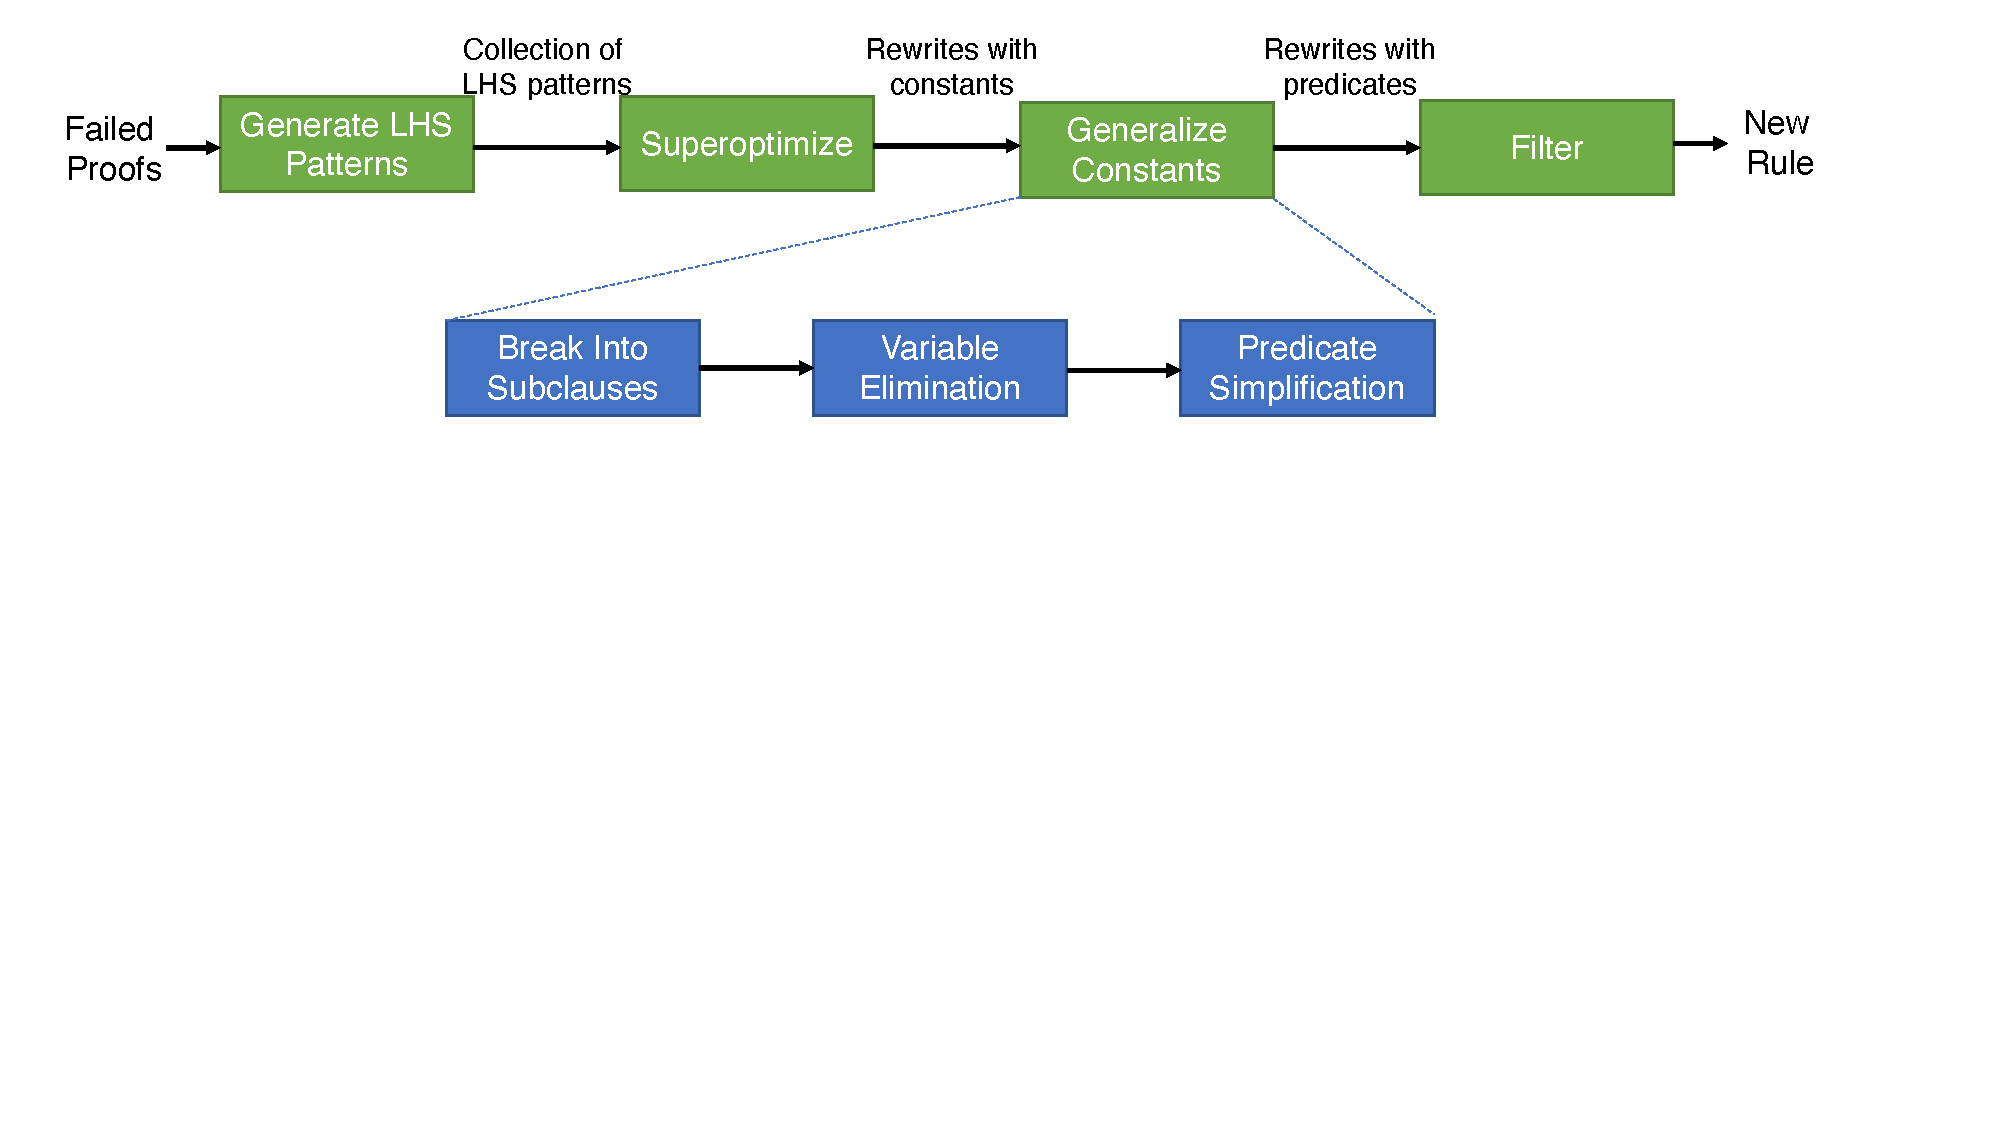
\includegraphics[width=1.9\columnwidth]{figures/synthesis-flow.pdf}
\caption{Overall flow of the synthesis pipeline.}
\label{fig:synthesis-flow}
\end{figure*}


The Halide term rewriting system is not complete: there
exist expressions checked by the compiler running on real-world pipelines that
the simplifier cannot resolve, but which are known to be true. \jln{there should
  be more discussion of TRS properties here (confluence etc) and whether they
  are decidable for the Halide lang} \sak{Julie: Can you add that please?}
In this section, we describe a workflow for automatically augmenting the Halide
TRS using program synthesis.
A high-level view of the synthesis pipeline is shown in Figure~\ref{fig:synthesis-flow}.
Overall, we begin by synthesizing candidate rules that contain concrete constants,
then generalize those rules by replacing concrete constants with wildcards that
match any compile-time constants, along with predicates checkable at compile-time
that encode constraints on those constants.

\subsection{Synthesizing Candidate Rules With Constants}
The aim of the synthesis pipeline is to learn new rules that would be of use in reasoning about input expressions.
For this work, scripts from the authors of \citeauthor{Adams2019}~\cite{Adams2019} that compiled
 random but realistic Halide pipelines with random schedules for
training the Halide autoscheduler. The compiler was instrumented to print expressions that the simplifier was unable to prove to be true, but that fuzz testing was not able to find to be false, a good indicator of a weak spot in the simplifier's reasoning power.
 For each failed proof, we attempt to generate one or more rules capable of transforming the expression.


\paragraph{Generating LHS Patterns} For a given failed expression, the first step
is to construct all left-hand-side patterns that match some portion of the expression.
We constrain the maximum length of a pattern to be six operations, to ensure fast matching
during term rewriting. At this stage, patterns preserve any constant values, and subtrees
that exactly match syntactically are assigned the same wildcard. For
example, given the expression $(a*b + c/b)$, where all nodes are non-constant,
we extract the following LHS patterns: $x + y$, $x * y$, $x / y$, $x * y + z$,
$x + y/z$, and $x*y + z/y$.  We then filter out any patterns that do not contain
a repeated wildcard, as such patterns are unlikely to result in a useful general
rewrite.  Thus, of the set above, we would only consider the last pattern, since
it contains a repeated $y$.  Although the set of candidate LHS patterns is exponential
in the size of the original expression, our filtering reduces the set to a tractable
size.

\paragraph{Synthesizing Right-Hand Sides} Given a candidate lefthand side, we 
synthesize a righthand side that is semantically equivalent and respects the reduction
order such that $\mathit{LHS} > \mathit{RHS}$.  We utilize two strategies for synthesizing
right-hand sides: reassociating and applying a known rewrite, or counter-example guided
inductive synthesis (CEGIS).

The first strategy comes from the insight that in many cases, rewrite rules would apply
if the expression were in a different form.  Therefore, we generate all possible
reassociations and commutations of the LHS expression, by unpacking the expression
into a flattened list of leaves, and then enumerating every valid binary
tree over permutations of the leaves that is semantically equivalent to the original
expression.  We then check whether an existing rule rewrites any enumerated reassociation.
When enumerating trees, we consider every reassociation and commutation
of associative and commutative node types, including addition and subtraction, max, and
min.  For non-associative/non-commutative nodes, we use the outer product of all reassociations
and commutations of their input arguments.  For example, the expression $(x/2 + y) - (x + 11)/2$
does not match an existing rewrite rule, but a reassociated version does: $y + (x/2 - (x + 11)/2)$
would be rewritten to $(-10 - (x \% 2)/2) + y)$.  Thus, we construct the candidate rewrite:
$$(x/2 + y) - (x + 11)/2 \equiv (-10 - (x \% 2)/2) + y)$$

If the first method fails, we apply CEGIS to superoptimize the lefthand side pattern.
We build a CEGIS loop on top of Z3~\cite{de2008z3}, encoding the LHS as a set of op codes
and searching for a semantically equivalent but shorter sequence of operations, similar
to prior work in superoptimization~\cite{regehr2018superoptimization, mangpo2016superoptimization}.
We first search for a single-op sequence,
than iteratively increase the number of operations, in order to find shorter sequences
first.  If CEGIS returns a sequence that is semantically equivalent to the LHS pattern but uses fewer
operations, it becomes the candidate RHS. Rather than try to encode the complex reduction order into the synthesis query itself, we use the op-code size of the synthesized expression as an approximation for the order

\paragraph{Limitations} While Z3 is a powerful tool for powering synthesis, we must take care to avoid
undecidable theories, in which case Z3 nearly always fails during the CEGIS process.
Therefore we limit the use of division and modulo in our op codes to be division
or modulo by 2 only, and rely on the generalization step described next to
widen the set of denominators for which a rule applies.  Because of this
restriction, our synthesized rules cannot contain non-constants in denominators
or the right hand side of a modulo.  As a result, our synthesis system cannot
construct all rules a human can.

\subsection{Generalizing Constants}

At this point in the synthesis pipeline, we have constructed a candidate rewrite
rule that contains concrete constants.  To make the rule as general as possible,
we replace each constant with a fresh \emph{constant variable}. A constant
variable matches only terms with constant values known at compile time. We first query Z3
again to see if the equivalence still holds; if it does, the rule is valid. If
it is not, we will need to find a \textit{predicate} to guard
applications of the rule in the simplifier. We attempt to synthesize a predicate
such that $pred \rightarrow LHS = RHS$ and all variables appearing in the
predicate are constant variables.

Consider the synthesized rule $c0 \cdot x > c1 \cdot x \equiv x > c2$, where $c0$, $c1$,
$c2$ are constant variables. We want to find some term $P$ such that
$P \rightarrow c0 \cdot x > c1 \cdot x \equiv x > c2$ and
$\mathcal{V}ar(P) \subseteq \{c0, c1, c2\}$. More generally, for a rule $R$, we begin by
negating $R$ and deriving as many facts from it as possible that refer only to
the constant variables. Once we have found $\neg R \rightarrow \neg P$, with $P$ containing
no non-constant variables, we know that $P \rightarrow R$, so $P$ serves as a
valid predicate for the rule.  For example, for the rule above, we derive implications
from $c0 \cdot x > c1 \cdot x \neq x > c2$, and then negate those implications to
construct the predicate.

Deriving facts that only contain constant variables requires applying variable
elimination to get rid of non-constant variables.  Our approach breaks up $\neg P$ into
a large number of simpler cases, then applies variable elimination to each case.

\paragraph{Dividing into Subclauses} We begin by subdividing a negated rewrite $l \neq r$ into
the cases $l \wedge \neg r$ and $\neg l \wedge r$.  We then further subdivide each case based
on the sign of any variables used in multiplication, division, or modulus, constructing
a case for negative, zero, or positive values of the variable (we skip the zero case for
division and modulo, because we assume no undefined behavior exists in the original expression).
For our example, we subdivide into three cases each for each of $c0$, $c1$, and $x$, yielding
54 cases.  We then further subdivide using any explicit conditionals in the expression (max,
min, and select), considering each branch separately.

Next, we introduce positive auxiliary variables ($k0..kn$ in our notation) to convert
inequalities into equalities, and remove all division and modulo operations using
variable substitutions.  After all these steps, we end up with a large number of simple
clauses in a conjuction.  For our example, one set of resulting clauses is:
\begin{align*}
c0 \cdot x = c1 \cdot x + k0  \wedge x + k1 = c2 & & \wedge \\
x > 0 \wedge
c0 > 0 \wedge 
c1 < 0 & & \wedge  \\
k0 \geq 1 \wedge k1 \geq 0 & &
\end{align*}

\paragraph{Variable Elimination} We employ three main strategies for eliminating
variables: traditional variable elimination, in which one equation is rewritten and
used to eliminate a variable in another equation; using reasoning over the signs in products;
and using Halide's bounds analysis machinery to find facts about the clauses.  The possible
set of manipulations is very large, and the non-linear nature of the systems prevent most
tools from robustly reasoning about the expressions.  To tractably eliminate variables and discover
facts about the systems, we use beam search~\cite{beamsearch} in order to avoid applying
all possible actions at each step.  Beam search uses a cost model to prune states, exploring
only the top $k$ scoring steps, and we hash states to avoid exploring the same state multiple
times.

We learn a cost model by featurizing systems of equations using a number of hand-crafted
features\footnote{The full set of features is: the number of constraints, number of variables,
  number of constant variables, the number of variables with known constant upper or lower bounds,
  the number of variables with known constant upper \textit{and} lower bounds, and the number of
  variables with known but non-constant upper or lower bounds.\sak{Check this list}},
and assigning a cost based on a linear combination of weights for each feature.  Initially,
we assign weights by hand, and then run on random systems of equations while keeping track
of which states led to eliminating a non-constant variable.  Then, we retrain the weights
as a logistic regressor that predicts which states will lead to successful elimination
by minimizing cross-entropy loss.  Interestingly, the regressor learned that the most
important feature is the one counting the number of constant variables, as our goal
is to eliminate only non-constant variables.  Perhaps unsurprisingly, the feature
with the largest negative coefficient was the number of unconstrained variables, as
these must be eliminated in order to make progress on the system overall.

The tree search logs all constraints found that only use constant variables.  Combining
these constraints and negating gives us the predicate $P$ we're searching for.

\subsection{Final Simplification \& Filtering} At this stage, we now have a candidate
rule and predicate over its constant variables.  However, the predicate is often quite
large and full of redundant clauses, which could make compile-time checks too slow.
We simplify the predicate by converting to conjunctive normal form (CNF) and applying
ad-hoc simplification rules that remove redundant terms.

After simplification, the predicate may still contain constraints on constant variables
that appear \textit{only on the right hand side}, since we never restricted which constant
variables can appear.  Thus, we must further transform the predicate to eliminate
constraints of this form.  Our strategy is to first try to transform a constant variable
$c$ into a form $c > Q$, $c < Q$, or $c = Q$ where $Q$ contains only constant variables
that appear on the LHS of the rule.  If this fails, we attempt further rewrites by
searching for any clause where $c$ is compared with any expression not containing RHS
constant variables.  If such a clause is found, we can rewrite $c$, but if not, the rule
cannot be checked at compile time and must be discarded.

Once we have a candidate rule guarded by a predicate, we perform three final checks.
First, we query Z3 to ensure the
predicate is satisfiable; if not, we discard the rule.  About 10\% of all rules fail
this filter.  Secondly, we check that the rule is not redundant.  For every pair of
rules $R_1$ and $R_2$, if $R_1$ matches every left hand side that $R_2$ matches,
and the predicate for $R_1$ implies the predicate for $R_2$, then we can discard $R_2$
as $R_1$ is at least as general. Finally, we check that the candidate rule obeys our
reduction order in order to preserve our termination guarantee. If the candidate rule passes all three filters, the rule can be added to the simplifier ruleset automatically without any human auditing.


\section{Evaluation}
In this section, we describe experiments to evaluate the improvements made to the Halide term rewriting system.  Specifically, we
test the following hypotheses:
\begin{enumerate}
\item Our improvements to the Halide TRS increases the robustness of the compiler and reduces compilation failures.
\item The improved TRS is more correct.
\item This improved robustness and correctness does not come at the cost of vastly slower compilation speed.
\item Our rule synthesis can be used to automate the effort of crafting new rules in response to bugs.
%\item Improving the TRS increases performance of generated code.
\end{enumerate}

We perform all experiments on (Andrew's machine: i9-9960X CPU @ 3.10GHz, Ubuntu 18.04, 16 threads using avx-512, LLVM 8.0.1).

\begin{figure}[htb]
  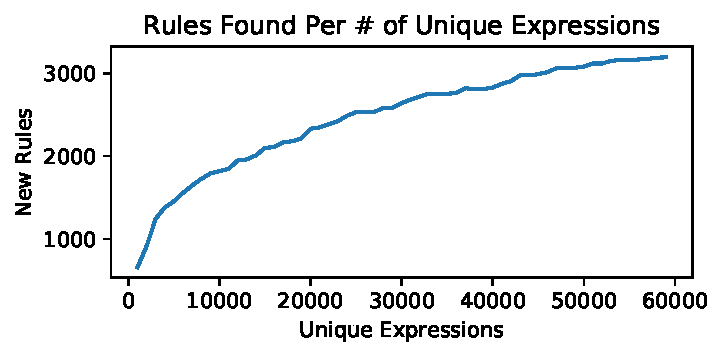
\includegraphics[width=\columnwidth]{figures/num-rules-found.pdf}
  \caption{The number of rules found as a function of unique failed expressions.  Initially, many new rules are discovered,
    but the rate begins to slow down after a few thousand expressions.}
  \label{fig:num-rules-found}
\end{figure}

Figure~\ref{fig:num-rules-found} shows the number of rules found as a function of the number of proof failures
examined.  At first, failed expressions yield many rules, but as expected, the number of rules found
begins to saturate after several thousand expressions.

\subsection{Robustness}
\begin{table*}[!ht]
  \caption{Proof failures before and after our improvements to the Halide term rewriting system.}
  \label{tab:simplifierfailures}
  \small
  {
\setlength\tabcolsep{2.5pt}
  \begin{tabular}{l|cc|cc|cc|cc|cc|cc|cc|cc|cc|cc}
& \multicolumn{2}{c|}{}  & \multicolumn{2}{c|}{local}  & \multicolumn{2}{c|}{}  & \multicolumn{2}{c|}{bilateral}  & \multicolumn{2}{c|}{camera}  & \multicolumn{2}{c|}{nl}  & \multicolumn{2}{c|}{stencil} & \multicolumn{2}{c|}{iir} & \multicolumn{2}{c|}{} & \multicolumn{2}{c}{max} \\
& \multicolumn{2}{c|}{harris}  & \multicolumn{2}{c|}{laplacian}  & \multicolumn{2}{c|}{unsharp}  & \multicolumn{2}{c|}{grid}  & \multicolumn{2}{c|}{pipe}  & \multicolumn{2}{c|}{means}  & \multicolumn{2}{c|}{chain} & \multicolumn{2}{c|}{blur} & \multicolumn{2}{c|}{interpolate} & \multicolumn{2}{c}{filter} \\
& new & old & new & old & new & old & new & old & new & old & new & old & new & old & new & old & new & old & new & old\\\hline
Proof failures & 6 & 6 & 10261 & 13569 & 19 & 18 & 51 & 54 & 1023 & 1089 & 117 & 133 & 7 & 7 & 1 & 1 & 254 & 301 & 1 & 0\\
\makecell[l]{Non-monotonic\\ expr} & 922 & 1605 & 11081 & 18539 & 1447 & 2232 & 2601 & 3993 & 9918 & 10795 & 621 & 3582 & 7352 & 18026 & 0 & 0 & 2008 & 5860 & 348 & 401\\\hline
\makecell[l]{Compile\\ time (min)} & 15.7 & 15.6 & 458.3 & 487.5 & 13.9 & 13.9 & 13.4 & 12.8 & 46.8 & 48.5 & 58.9 & 61.5 & 274.1 & 273.5 & 7.8 & 7.9 & 33.7 & 34.2 & 7.1 & 7.2\\
%Compile time (ms) & 2703 & 2637 & 136840 & 143032 & 2421 & 2386 & 2388 & 2327 & 14202 & 14097 & 20275 & 20607 & 90101 & 86976\\
%\% In Halide & 13\% & 	9\% & 	5\% & 	4\% & 	10\% & 	8\% & 	8\% & 	7\% & 	10\% & 	8\% & 	4\% & 	3\% & 	4\% & 	4\%\\
%\% In LLVM & 87\% & 	91\% & 	95\% & 	96\% & 	90\% & 	92\% & 	92\% & 	93\% & 	90\% & 	92\% & 	96\% & 	97\% & 	96\% & 	96\%\\
\end{tabular}
}

\end{table*}

Our hypothesis is that adding the newly synthesized rules to the Halide
simplifier has increased the set of expressions it can simplify. Since the
simplifier is non-confluent both before and after the new rules were added, we
have no theoretical guarantee that this is the case (in fact, it is possible
that the augmented simplifier might fail to simplify an expression that would
previously have succeeded if the new rules move the expression into a local
minimum). We test the robustness of the enhanced simplifier empirically by
compiling randomly generated schedules with the original and enhanced simplifier
and reporting the number of compilation failures.

Table~\ref{tab:simplifierfailures} summarizes the results.  Overall, the new rules
reduce the number of proof failures by 82\% and the number of non-monotonic expressions
by 44\%.  Interestingly, two of the test applications, unsharp and bilateral grid,
exhibit increases in simplifier failures of 44\% and 37\% respectively.  \sak{WHY?}


% could also report calls to can_prove and successful calls to can_prove; this is more meaningful as a ratio

\subsection{Correctness}
\label{sec:eval-correctness}
\begin{table*}

\caption{Incorrect rules found during verification.}
\begin{tabular}{|l|l|l|}
\hline
Incorrect rule & Counterexample & Tool used \\
\hline
$((x + c0)/c1)*c1 - x \rightarrow_R x \bmod c1 \textrm{ if } c1 > 0 \wedge c0 + 1 == c1$ & x := -2, c0 := 2, c1 := 3 & Z3 \\
$x - ((x + c0)/c1)*c1 \rightarrow_R -(x \bmod c1) \textrm{ if } c1 > 0 \wedge c0 + 1 == c1$ & x := -2, c0 := 2, c1 := 3 & Z3 \\
$min(x, c0) < min(x, c1) + c2 \rightarrow_R \textrm{false if } c0 >= c1 + c2)$ & x := 0, c0 := 0, c1 := -1, c2 := 1 & Z3 \\
$max(x, c0) < max(x, c1) + c2 \rightarrow_R \textrm{false if } c0 >= c1 + c2$ & x := 0, c0 := 2, c1 := 1, c2 := 1 & Z3 \\
\hline
\end{tabular}
\label{tab:incorrectrules}
\end{table*}



As described in Section~\ref{sec:soundness}, we improved the correctness of
the simplifier by verifying the existing rules using a combination of Z3 and
Coq. We ran our automated scripts on the 999 existing rewrite rules, using Z3
to verify 872 of them as correct.  We further verified 123 rules manually using
Coq.  We found \NumRulesFixed incorrect rules, shown in Table~\ref{tab:incorrectrules},
and submitted patches to the Halide developers. We also found
\NumPredicatesRelaxed rules whose predicates could be relaxed while retaining
correctness.

\sak{Write up the fact that we did in fact encounter a case where we
  synthesized a rule that resulted in infinite looping due to an existing
  ordering-violating rule}

We also ensure the termination of the simplifier by devising a reduction order
over its rewrite rules. We identify \NumOrderingProblems rewrite rules that do
not conform to this ordering, and reported them to the Halide developers. We generated 128 random schedules for each of our \NumApps, and evaluated performance with and without the \NumOrderingProblems rules, finding a negligible effect on runtime, which seems to indicate that removing the rules would give a termination guarantee without incurring a performance penalty.

% We also use this rule ordering to ensure we never create rules that violate the ordering, preventing infinite loops.
%We checked the existing Halide ruleset against our reduction order and found \NumOrderingProblems rules that were not properly ordered. We use the reduction order to ensure that the simplifier will always terminate by using the order to filter newly synthesized rules.
\subsection{Compilation Speed}
\label{ssec:compilationspeed}

We hypothesize that the Halide simplifier scales well in terms of the number of rewrite rules it uses, and thus adding synthesized rules will not greatly affect compilation times. We need empirical results to confirm this hypothesis, since adding rewrite rules could potentially improve simplification time for one expression and degrade it for another. If no rules match a given expression, the simplifier must try to match every applicable rule, so adding rules would increase simplification time; if a new rule allows the simplifier to make progress on a previously unsimplifiable rule, the simplifier will be able to continue working on the expression and thus take more steps. On the other hand, a new rule might allow an expression to simplify to a small expression quickly, thus reducing the number of rewrite steps the simplifier must take; furthermore, if the simplifier can now successfully prove a term when it could not before, it may be able to use some optimization, thus shortening (non-simplifier) compilation time overall.

We recorded the compilation times for the random schedules used in the robustness experiment above.

\jln{Ras suggests we record can\_prove expressions and get timing on simplifying them so we can separate simplifier timing from the full compliation times.}

%% \subsection{Generated Code Performance}

%% By increasing the robustness of the simplifier, we hypothesize that we increase the likelihood that the compiler will return more performant code. Halide ships with X sample applications; we compiled these applications with and without the newly synthesized rules and measured their runtime performance.

\subsection{Synthesizing Rules for Bugfixes}
\begin{table}
  \caption{Synthesizing rules for previous bugfixes.}
  \label{tab:prbugfixes}
  \begin{tabular}{lccc}
    PR ID & Rules Added & Synth. & Synth. Weaker\\
          & By Orig.    & Rules  & Rules\\\hline
    3780 & 2 & 0 & 2\\
    3770 & 5 & 3 & 1\\
    3765 & 10 & 9 & 0\\
    3761 & 8 & 8 & 0\\
    3719 & 1 & 0 & 0\\
  \end{tabular}
\end{table}
Many modifications to the term rewriting system occur in response to user-reported
miscompilations or other bugs.  Crafting rewrite rules for fixing a specific misbehavior
is tedious and error-prone; comments from commits to the Halide repository include
``Proving these rules on paper is a pain.''  For this experiment, we explore whether
our automated rule synthesis can replace the human effort.  We look at the last 5 pull
requests in the Halide git repository~\footnote{https://github.com/halide/Halide} that add rules.  Then, we remove
the added rules and use either tests from the PR or hand-crafted failures (in rules
not exercised by the added tests) and pass them to our system.
Table~\ref{tab:prbugfixes} summarizes results from the experiment.

Our automated system derives 23 new rules, while humans added 26 rules.  Of the three
rules the synthesizer failed to create, two were due to being outside the search scope
of the synthesizer: one (PR 3719) only operated on vectors, and the other (in PR 3770) was $x \% x = 0$, which
performs modulo without a constant so is not within our grammar.  Of the 23 successful
rules, two (from PR 3780) were less general because the synthesized rule only allowed division
or modulo by a constant, while the original bugfix applies to constants or variables.
In that specific case, a rule that pulls a division out of a select statement
is synthesized so that the divisor is a non-zero constant, and similarly for modulo.

Overall, the experiment shows that real-world bugfixes can be synthesized by
our system, replacing much of the tedious human effort required when crafting
new rules by hand.

\section{Limitations}
Synthesis oracle (z3) can't reason about expressions with div/mod, so we're limited in our ability to synthesize those types of rules.

Integers only, no floats etc.

Overflows not considered.

\section{Future work}
The Halide simplifier is used both to prove expressions true or false and to simplify expressions to more easily optimizable forms, but these two usecases are not always aligned. One could imagine two separate simplifiers with different rulesets and reduction orders. One interesting direction for future work might be to use the synthesizer to create these two rulesets, which would otherwise be a very human-effort intensive task.

Although we do not currently synthesize rules that contain vector operators, they are not incompatible with our approach. Since our reduction of Halide expressions to SMT formulas models vector expressions as integers, we would need to add a typechecking step to ensure correctness in the synthesis process, which we leave as future work.

The priority in which rules are considered for matching clearly can have performance implications, but evaluation/tuning is left as future work.

\section{Related Work}

Program synthesis has been applied to term rewriting systems in Swapper~\cite{singh2016swapper}, a tool that learns a set of rewrite formulas to transform SMT formulas into forms that can be more easily solved by theory solvers. Swapper takes a training set of formulas drawn from a target domain, does probabilistic sampling to choose LHS candidates, synthesizes predicates and RHS, and finally autotunes the resulting ruleset to choose a rule subset and rule order that gives the best solver performance. Unlike our work, Swapper is an optimizer rather than a prover. Because our rewrite algorithm scales well in terms of the number of rules, we simply use all candidate LHS terms for synthesis rather than sampling. Swapper synthesizes RHS terms that have fewer AST nodes than their corresponding LHS terms; this is not a reduction order and does not guarantee termination, although the autotuning step should reject rulesets with cycles. Finally, Swapper creates a fresh term rewriting system with each invocation, whereas our work augments and maintains an existing term rewriting system.

Butler et al.~\cite{butler2017synthesizing} uses synthesis to learn human-interpretable strategies for puzzle games such as Sudoku or Nonograms. Strategies consist of a pattern (LHS term with variables), condition (predicate), and action (RHS term expressing rewrite), and so comprise a term rewriting system. Strategies are synthesizing Rosette, using a CEGIS loop similar to our synthesis process. Progress in these puzzle games is always monotonic, which gives a natural reduction order. Their goal is to model human strategies, which are greedy and non-deterministic, so they do not consider rule priority or any particular term rewriting algorithm. 

Herbie, superoptimization, abstract interpretation, MCSAT (Jovanovic)

\section{Conclusion}


%% Acknowledgments
\begin{acks}                            %% acks environment is optional
                                        %% contents suppressed with 'anonymous'
  %% Commands \grantsponsor{<sponsorID>}{<name>}{<url>} and
  %% \grantnum[<url>]{<sponsorID>}{<number>} should be used to
  %% acknowledge financial support and will be used by metadata
  %% extraction tools.
  This material is based upon work supported by the
  \grantsponsor{GS100000001}{National Science
    Foundation}{http://dx.doi.org/10.13039/100000001} under Grant
  No.~\grantnum{GS100000001}{nnnnnnn} and Grant
  No.~\grantnum{GS100000001}{mmmmmmm}.  Any opinions, findings, and
  conclusions or recommendations expressed in this material are those
  of the author and do not necessarily reflect the views of the
  National Science Foundation.
\end{acks}


%% Bibliography
\bibliography{bib}


%% Appendix
\appendix
\section{Appendix}

\subsection{Halide expression grammar}
\label{ss:appendixA}


\begin{grammar}
<Expr> ::= <BoolExpr> 
\alt <IntExpr> 
\alt <VectorExpr>

<BoolExpr> ::= `true'
\alt `false'
\alt <IntExpr> `<' <IntExpr>
\alt <IntExpr> `>' <IntExpr>
\alt <IntExpr> `<=' <IntExpr>
\alt <IntExpr> `>=' <IntExpr>
\alt <IntExpr> `=' <IntExpr>
\alt <IntExpr> `!=' <IntExpr>
\alt <VectorExpr> `<' <VectorExpr>
\alt <VectorExpr> `>' <VectorExpr>
\alt <VectorExpr> `<=' <VectorExpr>
\alt <VectorExpr> `>=' <VectorExpr>
\alt <VectorExpr> `=' <VectorExpr>
\alt <VectorExpr> `!=' <VectorExpr>
\alt <BoolExpr> `&&' <BoolExpr>
\alt <BoolExpr> `||' <BoolExpr>
\alt `!' <BoolExpr>

<IntExpr> ::= <IntExpr> `+' <IntExpr>
\alt <IntExpr> `-' <IntExpr>
\alt <IntExpr> `*' <IntExpr>
\alt <IntExpr> `/' <IntExpr>
\alt <IntExpr> `\%' <IntExpr>
\alt `max' <IntExpr> <IntExpr>
\alt `min' <IntExpr> <IntExpr>
\alt `select' <BoolExpr> <IntExpr> <IntExpr>
\alt integers

<VectorExpr> ::= `broadcast' <IntExpr>
\alt `ramp' <IntExpr> <IntExpr>
\alt <VectorExpr> `+' <VectorExpr>
\alt <VectorExpr> `-' <VectorExpr>
\alt <VectorExpr> `*' <VectorExpr>
\alt <VectorExpr> `/' <VectorExpr>
\alt <VectorExpr> `\%' <VectorExpr>
\alt `max' <VectorExpr> <VectorExpr>
\alt `min' <VectorExpr> <VectorExpr>
\alt `select' <BoolExpr> <VectorExpr> <VectorExpr>
\end{grammar}

\subsection{The full Halide reduction order}
\label{a:reductionorder}

For some term $s \in T(\Sigma, V)$ and some variable $x \in V$, let $|s|_x$ be the number occurrences of the variable $x$ in the term $s$.

Let $\mathcal{P}os(t)$ be the set of indexes to the subterms in the term $t$, and let $t|_p$ be a subterm of the term $t$ at the position $p$. Then, $s >_{vec} t$ iff the number of occurrences of \texttt{ramp} and \texttt{broadcast} in $s$ are greater than the number of occurrences in $t$ and that for every variable contained by $t$, if it is present in some subterm $t|_p$ and that subterm does not start with a \texttt{ramp} or \texttt{broadcast}, then the number of occurrences of that variable must be greater or equal in $s$ than in $t$.

\begin{gather*}
%\begin{split}
s >_{vec} t \iff \\
 |s|_{\texttt{ramp}} + |s|_{\texttt{broadcast}} > |t|_{\texttt{ramp}} + |t|_{\texttt{broadcast}} \wedge \\
\forall x \in V, (\exists p \in \mathcal{P}os(t), x \in t|_p \wedge \\
(t|_p \neq \texttt{ramp}(v_1,v_2) \wedge t|_p \neq \texttt{broadcast}(v))) \\
\implies |s|_x \geq |t|_x
%\end{split}
\end{gather*}

Next, $s >_{var} t$ iff for every variable that occurs in $t$, it occurs strictly more times in $s$.

\begin{equation*}
s >_{var} t \iff \forall x \in \mathcal{V}ar(t), |s|_x > |t|_x
\end{equation*}

We say $s >_{nonlinear} t$ if the total number of multiplications, divisions, and moduluses in $s$ is greater than that of $t$, while all variables in $t$ occur an equal or greater number of times in $s$.

\begin{equation}
\begin{split}
s >_{nonlinear} t \iff \forall x \in \mathcal{V}ar(t), |s|_x \geq |t|_x \wedge \\
\sum_{op \in \{*,/,\%\}} |s|_{op} > \sum_{op \in \{*,/,\%\}} |t|_{op}
\end{split}
\end{equation}

We say $s >_{op} t$ if the total number of all operations in $s$ is greater than that of $t$, while all variables in $t$ occur an equal or greater number of times in $s$.

\begin{equation}
\begin{split}
s >_{op} t \iff \forall x \in \mathcal{V}ar(t), |s|_x \geq |t|_x \wedge \\
\sum_{op \in \Sigma} |s|_{op} > \sum_{op \in \Sigma} |t|_{op}
\end{split}
\end{equation}

The next order is itself a lexicographic composition of a series of orders over total counts of each type of operation, using the order specified in ~\ref{symbolstrength}; first terms are compared by the number of \texttt{ramp} occurrences; if those are equal they are compared by the number of \texttt{broadcast} operators, and so on. 

\begin{equation}
\begin{split}
s >_{histo} t \iff \forall x \in \mathcal{V}ar(t), |s|_x \geq |t|_x \wedge \\
|s|_{\texttt{ramp}} > |t|_{texttt{ramp}} \vee \\
|s|_{\texttt{ramp}} = |t|_{texttt{ramp}} \wedge |s|_{\texttt{broadcast}} > |t|_{texttt{broadcast}} \vee \\
\dots \\
\dots \wedge |s|_{\texttt{=}} > |t|_{texttt{=}} 
\end{split}
\end{equation}

The last two orders are recursive multiset path orders, defined in general as:

\begin{equation}
\begin{split}
s >_{mpo} t \iff & t \in \mathcal{V}ar(s) \vee \\
              &  s = f(s_1,\dots,s_m), t = g(t_1,...,t_n), f > g \vee \\
               & \{s_1, \dots, s_m\} >_{mpo} \{t_1,\dots,t_n\}
\end{split}
\end{equation}

First, $s >_{mpo^+} t$ where $>_mpo^+$ is a multiset path order defined on the strict order $<_+$ over all Halide operators.

\begin{equation}
f >_+ g \iff (f \neq \texttt{+} \wedge f \neq \texttt{-}) \wedge (g = \texttt{+} \vee g = \texttt{-})
\end{equation}

\[
f_{root_{\texttt{+}}}(term) = \begin{cases}
                          1 & root(term) \neq \texttt{+} \wedge root(term) \neq \texttt{-} \\
                          0 & otherwise
                          \end{cases}
\]

\begin{equation}
s >_{root_{\texttt{+}}} t \iff f_{root_{\texttt{+}}}(s) > f_{root_{\texttt{+}}}(t)
\end{equation}

Finally, $s >_{mpo^{op}} t$ where $>_{mpo^{op}}$ is a multiset path order defined on a strict order over the Halide operators as defined in ~\ref{symbolstrength}.

\subsection{Halide symbol strength} \label{symbolstrength}

The function symbols in the Halide expression signature, in order by strength, greatest to least.

\begin{enumerate}
  \item \texttt{ramp}
  \item \texttt{broadcast}
  \item \texttt{select}
  \item \texttt{/}
  \item \texttt{*}
  \item \texttt{$\%$}
  \item \texttt{+, -} (equal strength)
  \item \texttt{max, min} (equal strength)
  \item \texttt{!}
  \item \texttt{||}
  \item \texttt{$\&\&$}
  \item \texttt{$>=$}
  \item \texttt{$>$}
  \item \texttt{$<=$}
  \item \texttt{$<$}
  \item \texttt{$!=$}
  \item \texttt{=}
\end{enumerate}

\end{document}
